%%%%%%%%%%%%%%%%%%%%%%%%%%%%%%%%%%%%%%%%%
% Jacobs Landscape Poster
% LaTeX Template
% Version 1.0 (29/03/13)
%
% Created by:
% Computational Physics and Biophysics Group, Jacobs University
% https://teamwork.jacobs-university.de:8443/confluence/display/CoPandBiG/LaTeX+Poster
% 
% Further modified by:
% Nathaniel Johnston (nathaniel@njohnston.ca)
%
% This template has been downloaded from:
% http://www.LaTeXTemplates.com
%
% License:
% CC BY-NC-SA 3.0 (http://creativecommons.org/licenses/by-nc-sa/3.0/)
%
%%%%%%%%%%%%%%%%%%%%%%%%%%%%%%%%%%%%%%%%%

%----------------------------------------------------------------------------------------
%	PACKAGES AND OTHER DOCUMENT CONFIGURATIONS
%----------------------------------------------------------------------------------------

\documentclass[final]{beamer}

\usepackage[scale=1.24]{beamerposter} % Use the beamerposter package for laying out the poster

\usetheme{confposter} % Use the confposter theme supplied with this template

%https://tex.stackexchange.com/questions/252354/sum-symbol-in-tikzposter-too-small
%\usepackage[utf8]{inputenc}
\usepackage{graphicx}
\usepackage[T1]{fontenc} 
\usepackage{lmodern} 
\usepackage{amsmath}
\usepackage{amssymb}
\usepackage{textcomp}
%\DeclareUnicodeCharacter{00A0}{ }

% declare `cmex` to be arbitrary scalable
\DeclareFontShape{OMX}{cmex}{m}{n}{
	<-7.5> cmex7
	<7.5-8.5> cmex8
	<8.5-9.5> cmex9
	<9.5-> cmex10
}{}

\SetSymbolFont{largesymbols}{normal}{OMX}{cmex}{m}{n}
\SetSymbolFont{largesymbols}{bold}  {OMX}{cmex}{m}{n}

\setbeamercolor{block title}{fg=ngreen,bg=white} % Colors of the block titles
\setbeamercolor{block body}{fg=black,bg=white} % Colors of the body of blocks
\setbeamercolor{block alerted title}{fg=white,bg=UVicdarkblue} % Colors of the highlighted block titles dblue!70
\setbeamercolor{block alerted body}{fg=black,bg=dblue!10} % Colors of the body of highlighted blocks
% Many more colors are available for use in beamerthemeconfposter.sty

%-----------------------------------------------------------
% Define the column widths and overall poster size
% To set effective sepwid, onecolwid and twocolwid values, first choose how many columns you want and how much separation you want between columns
% In this template, the separation width chosen is 0.024 of the paper width and a 4-column layout
% onecolwid should therefore be (1-(# of columns+1)*sepwid)/# of columns e.g. (1-(4+1)*0.024)/4 = 0.22
% Set twocolwid to be (2*onecolwid)+sepwid = 0.464
% Set threecolwid to be (3*onecolwid)+2*sepwid = 0.708

\newlength{\sepwid}
\newlength{\onecolwid}
\newlength{\twocolwid}
\newlength{\threecolwid}
\setlength{\paperwidth}{48in} % A0 width: 46.8in
\setlength{\paperheight}{36in} % A0 height: 33.1in
\setlength{\sepwid}{0.024\paperwidth} % Separation width (white space) between columns
\setlength{\onecolwid}{0.22\paperwidth} % Width of one column
\setlength{\twocolwid}{0.464\paperwidth} % Width of two columns
\setlength{\threecolwid}{0.708\paperwidth} % Width of three columns
\setlength{\topmargin}{-0.5in} % Reduce the top margin size
%-----------------------------------------------------------

\usepackage{graphicx}  % Required for including images

\usepackage{booktabs} % Top and bottom rules for tables

%----------------------------------------------------------------------------------------
%	TITLE SECTION 
%----------------------------------------------------------------------------------------

\title{Renewable Energy Systems with Battery Storage: An Alberta Case Study} % Poster title

\author{Adam McKenna, Jon Duan and G. Cornelis van Kooten} % Author(s)

\institute{Department of Economics -  University of Victoria} % Institution(s)Department and University Name

%----------------------------------------------------------------------------------------

\begin{document}

\addtobeamertemplate{block end}{}{\vspace*{2ex}} % White space under blocks
\addtobeamertemplate{block alerted end}{}{\vspace*{2ex}} % White space under highlighted (alert) blocks

\setlength{\belowcaptionskip}{2ex} % White space under figures
\setlength\belowdisplayshortskip{2ex} % White space under equations

\begin{frame}[t] % The whole poster is enclosed in one beamer frame

\begin{columns}[t] % The whole poster consists of three major columns, the second of which is split into two columns twice - the [t] option aligns each column's content to the top

\begin{column}{\sepwid}\end{column} % Empty spacer column

\begin{column}{\onecolwid} % The first column

%----------------------------------------------------------------------------------------
%	OBJECTIVES
%----------------------------------------------------------------------------------------

\begin{alertblock}{Objectives}

To investigate the potential to use battery storage to meet Alberta's goal of eliminating reliance on coal power  and replacing coal with renewables.
\begin{itemize}
\item Integrate wind and solar energy into grid
\item Two levels of carbon tax are considered
\item All coal-fired plants are phased out  
\item Combined-cycle natural gas (CC gas) for base load
\item Li-ion batteries use cases for the transmission system or peak-replacement applications
\end{itemize}

\end{alertblock}

%----------------------------------------------------------------------------------------
%	INTRODUCTION
%----------------------------------------------------------------------------------------

\begin{block}{Introduction}

Alberta will phase out all coal-fired power plants and replace two-thirds of the lost electricity production with renewables by 2030. 

\begin{enumerate}
	\item The investment of renewables is incentivized by a \textbf{carbon tax} of \$20/t $CO_2$ beginning January 2017, followed by an increase to \$30/t $CO_2$ a year later.   
	
	\item The renewables such as wind and solar are \textbf{intermittent}. The wind may stop quickly, the sun may not shine suddenly, and the energy from renewables is not stable and reliable.  
	
	\item With the 30\% penetrate rate of intermittent renewables, some form of energy storage technology will be needed to maintain a reliable power supply throughout the province. 
	
	\item This paper investigates the relative costs and benefits of various types of policies aimed at eliminating coal-fired power and incentivizing the integration of renewables into the Alberta grid.
\end{enumerate}
%------------------------------------------------

\begin{figure}
	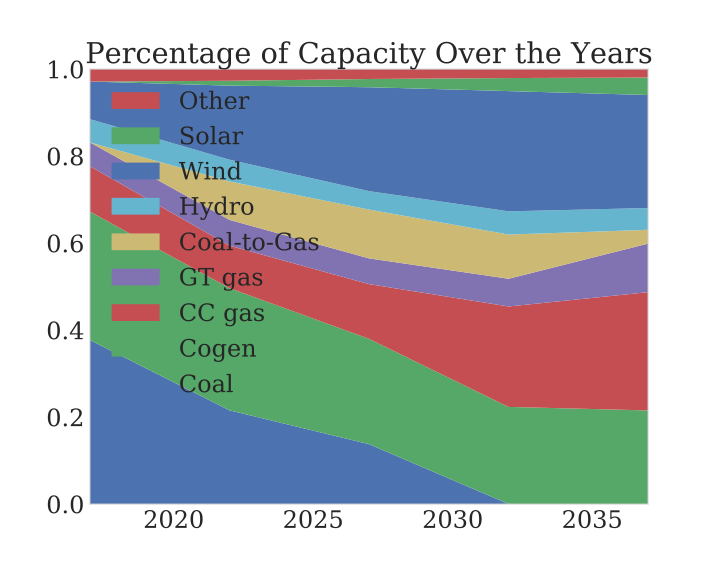
\includegraphics[width=0.9\linewidth]{capacity}
	\caption{Alberta's goal}
\end{figure}


\end{block}


%----------------------------------------------------------------------------------------

\end{column} % End of the first column

\begin{column}{\sepwid}\end{column} % Empty spacer column

\begin{column}{\twocolwid} % Begin a column which is two columns wide (column 2)

\begin{columns}[t,totalwidth=\twocolwid] % Split up the two columns wide column

\begin{column}{\onecolwid}\vspace{-.6in} % The first column within column 2 (column 2.1)

%----------------------------------------------------------------------------------------
%	MATERIALS
%----------------------------------------------------------------------------------------

\begin{block}{Data}

The following materials were required to complete the research:

\begin{itemize}
	
\item Hourly \textbf{load} data from 2005 to 2016 from Alberta Electric System Operator (\textbf{AESO})

\item Hourly \textbf{wind} speed data for 17 locations 2006 to 2015 from Government of Canada

 \begin{itemize}
	\item used to simulate the output of a 3.5 MW turbine
\end{itemize}

\item Hourly \textbf{solar} data for 28 locations 1996 to 2005 from Canadian Weather Energy and Engineering Datasets (\textbf{CWEEDS})

 \begin{itemize}
	\item used to simulate the output of a Solar Module
\end{itemize}

\end{itemize}

%------------------------------------------------

\begin{figure}
	\includegraphics[width=0.8\linewidth]{load_rad}
	\caption{Average Load and Solar Irradiance in January}
\end{figure}


\end{block}





%----------------------------------------------------------------------------------------
%	METHODS
%----------------------------------------------------------------------------------------

\begin{block}{Methodology}
	
\textbf{Optimization:}


AESO minimizes total cost by choosing: 
	\begin{itemize}
		\item the amount of wind turbines and solar panels
		\item the size of lithium-ion battery and the flow of energy into and out of the battery in each hour
		\item the overall capacity of gas generation and the hourly production of electricity from natural gas
	\end{itemize}
	

	
\textbf{Scenarios:}
	
	\begin{itemize}
		\item Different profiles wind and solar energy
		    \begin{itemize}
		    	\item each year of solar, wind and load data as a representative year 
		    \end{itemize}
		\item Different levels of carbon tax 
		
		\begin{itemize}
			\item \$0/t $CO_2$;  \$20/t $CO_2$ ;   \$30/t $CO_2$
		\end{itemize}
		
		\item Different use case of battery
		
		\begin{itemize}
			\item Transmission system (provide voltage support and grid stabilization, etc) ; Peaker replacement(replace peaking gas turbine facilities)
		\end{itemize}
	\end{itemize}
	
	
\end{block}




%----------------------------------------------------------------------------------------

\end{column} % End of column 2.1

\begin{column}{\onecolwid}\vspace{-.6in} % The second column within column 2 (column 2.2)


%----------------------------------------------------------------------------------------
%	MATHEMATICAL SECTION
%----------------------------------------------------------------------------------------

\begin{block}{Optimization}

\textbf{Objective:}

\begin{equation}
TC = \sum_{r \in \{w,s\}} \sum_{t=1}^{T} C_r N_r P_{r,t} +  \sum_{t=1}^{T} C_g P_{g,t} + C_b \times K_b
\label{eqn:objective}
\end{equation}

\begin{itemize}
	\item TC refers to the total cost of the hybrid renewable energy system
	\item $C_i, \quad i \in \{w, s, g, b\}$ refer to exogenous the levelized costs of electricity (LCOE) of renewable wind(w) and solar(s), natural gas(g) and battery storage(b); 
	\item $N_w$ and $N_s$ refer to the number of wind turbines and solar modules to be installed
	\item $P_{r,t}$ refers to the amount of energy produced by each renewable unit $N_r, r \in \{w, s\}$
	\item $b$ refers to the energy rating of the battery (MWh)

\end{itemize}


\textbf{Constraints:}

\begin{equation}
\displaystyle \sum_{r \in \{w,s\}}  N_r P_{r,t} + P_{g,t} + b_t^{-} \ge D_t + b_t^{+} 
\label{eq:demand}
\end{equation}

\begin{itemize}
	\item $b_t^{-}$   the discharge from the battery at time $t$ to meet demand 
	\item  $b_t^{+}$  the flow of energy into the battery (charge) at time $t$ if there is too much power available
\end{itemize}



\begin{equation}
V_{b,t}  =  V_{b,t+1} + \delta b_{t-1}^{+} - b_{t-1}^{-} 
\label{eq:battery}
\end{equation}


\begin{itemize}
	\item $\delta = 0.92$ is the round trip efficiency of the battery
	\item Dynamic equation that indicates the available energy in the battery at time $t$ 
\end{itemize}


\begin{equation}
b_t^{-} \le  V_{b,t} 
\label{eq:discharge}
\end{equation}

\begin{itemize}
	\item Discharge from the battery cannot exceed the current energy available in the battery
\end{itemize}


\begin{equation}
P_{g,t} \le  G 
\label{eq:gas}
\end{equation}

\begin{itemize}
	\item Power produced by a gas turbine cannot exceed its capacity 
\end{itemize}

\end{block}




%----------------------------------------------------------------------------------------

\end{column} % End of column 2.2

\end{columns} % End of the split of column 2 - any content after this will now take up 2 columns width

%----------------------------------------------------------------------------------------
%	IMPORTANT RESULT
%----------------------------------------------------------------------------------------

%\begin{alertblock}{Important Result}
%
%Lorem ipsum dolor \textbf{sit amet}, consectetur adipiscing elit.sapien ac commodo. Donec ut volutpat elit.
%
%\end{alertblock} 




%----------------------------------------------------------------------------------------

%\begin{columns}[t,totalwidth=\twocolwid] % Split up the two columns wide column again

%\begin{column}{\onecolwid} % The first column within column 2 (column 2.1)

%----------------------------------------------------------------------------------------

%\end{column} % End of column 2.1

%\begin{column}{\onecolwid} % The second column within column 2 (column 2.2)



%----------------------------------------------------------------------------------------

%\end{column} % End of column 2.2

%\end{columns} % End of the split of column 2

\end{column} % End of the second column

\begin{column}{\sepwid}\end{column} % Empty spacer column

\begin{column}{\onecolwid} % The third column
	
	


%----------------------------------------------------------------------------------------
%	RESULTS
%----------------------------------------------------------------------------------------

\begin{block}{Results}
	
\begin{enumerate}
	\item Without carbon levies, CC gas supplies electricity all of the time, as it has the \textbf{lowest LCOE} 
    \item With lower level of carbon levy, wind power is \textbf{integrated} into the system; however, the battery \textbf{utilization rate} remains low throughout, and only be used 0.5\% of the time
    \item With higher level of carbon levy, installed wind capacity \textbf{increases}; the battery utilization factor increases as well
    \item Solar power was not found to be optimal in any of simulations; its relatively \textbf{higher LCOE} remains a barrier to entry
    \item In many time periods, more energy was produced than needed; it would not be optimal for battery capacities to be so high as to capture all the wasted renewable energy, all the time. 
\end{enumerate}
%	
%	\begin{table}
%		\vspace{2ex}
%		\begin{tabular}{l l l}
%			\toprule
%			\textbf{Treatments} & \textbf{Response 1} & \textbf{Response 2}\\
%			\midrule
%			Treatment 1 & 0.0003262 & 0.562 \\
%			Treatment 2 & 0.0015681 & 0.910 \\
%			Treatment 3 & 0.0009271 & 0.296 \\
%			\bottomrule
%		\end{tabular}
%		\caption{Table caption}
%	\end{table}
	
\end{block}

	

%----------------------------------------------------------------------------------------
%	CONCLUSION
%----------------------------------------------------------------------------------------

\begin{alertblock}{Conclusion}

As renewable and battery \textbf{cost} continue to drop, Alberta may see itself relying \textbf{more} on wind and natural gas in its generation mix, and batteries may be hypothesised to replace conventional gas turbines as peakers in the near future. 

\end{alertblock}

%----------------------------------------------------------------------------------------
%	ADDITIONAL INFORMATION
%----------------------------------------------------------------------------------------

\begin{block}{Additional Information}

Our simulation merely captures the \textbf{monetary} aspects of renewable integration and energy storage, while ignoring many of the benefits that can accrue from such projects.

\end{block}

%----------------------------------------------------------------------------------------
%	REFERENCES
%----------------------------------------------------------------------------------------

%\begin{block}{References}
%
%\nocite{*} % Insert publications even if they are not cited in the poster
%\small{\bibliographystyle{unsrt}
%\bibliography{sample}\vspace{0.75in}}
%
%\end{block}

%----------------------------------------------------------------------------------------
%	ACKNOWLEDGEMENTS
%----------------------------------------------------------------------------------------

%\setbeamercolor{block title}{fg=ngreen,bg=white} % Change the block title color
%
%\begin{block}{Acknowledgements}
%
%\small{\rmfamily{Nam mollis tristique neque eu luctus. Suspendisse rutrum congue nisi sed convallis. Aenean id neque dolor. Pellentesque habitant morbi tristique senectus et netus et malesuada fames ac turpis egestas.}} \\
%
%\end{block}

%----------------------------------------------------------------------------------------
%	CONTACT INFORMATION
%----------------------------------------------------------------------------------------

\setbeamercolor{block alerted title}{fg=black,bg=norange} % Change the alert block title colors
\setbeamercolor{block alerted body}{fg=black,bg=white} % Change the alert block body colors

\begin{alertblock}{Contact Information}

\begin{itemize}
\item Web: \href{https://web.uvic.ca/~repa/}{https://web.uvic.ca/~repa/}
\item Email: \href{mailto:jonduan@uvic.ca}{jonduan@uvic.ca}
%\item Phone: +1 (000) 111 1111
\end{itemize}

\end{alertblock}

\begin{center}
\begin{tabular}{ccc}
\includegraphics[width=0.9\linewidth]{ECON_comb_h_4c.eps} %& \hfill & %\includegraphics[width=0.4\linewidth]{logo.png}
\end{tabular}
\end{center}

%----------------------------------------------------------------------------------------

\end{column} % End of the third column

\end{columns} % End of all the columns in the poster

\end{frame} % End of the enclosing frame

\end{document}
